\documentclass[10pt]{beamer}

% Tema Limpo e Profissional
\usetheme{Madrid}
\usecolortheme{whale}

% Pacotes Essenciais
\usepackage[utf8]{inputenc}
\usepackage[portuguese]{babel}
\usepackage{graphicx}
\usepackage{booktabs}
\usepackage{amsmath}
\usepackage{amssymb}
\usepackage{listings}
\usepackage{xcolor}

% Configuracoes de Codigo (Python)
\lstset{
    language=Python,
    basicstyle=\ttfamily\tiny,
    keywordstyle=\color{blue},
    stringstyle=\color{red},
    commentstyle=\color{green!60!black},
    breaklines=true,
    showstringspaces=false
}

% Metadados com Prevencao de Avisos de Metadados PDF
\title[ADS - Aula 11]{Testes de Hipótese e Permutação}
\subtitle{Ciência de Dados e Decisão}
\author[Reginaldo Fernandes]{Prof. Reginaldo Fernandes\texorpdfstring{\\ \small{Adaptação Didática}}{}}
\institute[IFCE]{Instituto Federal do Ceará -- Campus Tauá \\ Tecnologia em Análise e Desenvolvimento de Sistemas}
\date{\today}

\begin{document}
\begin{frame}\titlepage\end{frame}
\begin{frame}{Sumario da Aula}\tableofcontents\end{frame}

% Blocos Modulares de Slides
\section{Introdução e Estudo de Caso (Swain vs. Alabama)}

\begin{frame}{O Problema da Decisão com Dados}
    \begin{block}{Pergunta Fundamental}
        Como avaliar se uma discrepância observada em nossos dados é real (sinal sistemático) ou se é apenas fruto da variabilidade natural do acaso (ruído aleatório)?
    \end{block}
    \begin{block}{Exemplos Anteriores}
        \begin{itemize}
            \item Eficácia de vacinas em ensaios clínicos.
            \item Probabilidade em lançamentos de moedas.
            \item Diferença de peso de recém-nascidos.
        \end{itemize}
    \end{block}
    \centering
    \textit{Hoje exploraremos uma abordagem computacional robusta baseada em simulação e reamostragem para responder a essa pergunta de forma intuitiva.}
\end{frame}

\begin{frame}{Estudo de Caso: Robert Swain vs. Alabama (1962)}
    \begin{block}{O Contexto Histórico}
        Em 1962, Robert Swain, um homem negro, foi condenado à morte no Alabama. Ele apelou da sentença apontando que o júri era inteiramente branco e denunciou discriminação racial sistemática no processo de seleção.
    \end{block}
    \begin{columns}
        \begin{column}{0.6\textwidth}
            \textbf{Dados Demográficos do Caso:}
            \begin{itemize}
                \item População de jurados elegíveis: $26\%$ negros.
                \item Painel de pré-seleção ($N$): $100$ homens.
                \item Quantidade de negros no painel ($X$): apenas $8$ ($8\%$).
                \item Júri final da condenação: $0$ negros.
            \end{itemize}
        \end{column}
        \begin{column}{0.4\textwidth}
            \centering
            \textit{A Suprema Corte americana negou o apelo afirmando que a discrepância era pequena.}
        \end{column}
    \end{columns}
\end{frame}

\begin{frame}{Relembrando: Intervalo de Confiança Clássico (TCL)}
    \begin{columns}
        \begin{column}{0.5\textwidth}
            \begin{block}{Parâmetros da Amostra}
                \begin{itemize}
                    \item $N = 100$ jurados.
                    \item $p = 0.08$ ($8\%$ negros).
                \end{itemize}
            \end{block}
            \begin{block}{Variância de Bernoulli}
                $X_i \in \{0, 1\}$ (V.A. de Bernoulli):
                \begin{itemize}
                    \item Média ($\bar{X}$) = $p = 0.08$
                    \item Variância ($s^2$) = $p(1 - p) = 0.0736$
                    \item Erro Padrão ($SE$) = $\sqrt{\frac{p(1 - p)}{N}} \approx 0.0271$
                \end{itemize}
            \end{block}
        \end{column}
        \begin{column}{0.5\textwidth}
            \begin{alertblock}{Cálculo do $IC_{95\%}$ via TCL}
                $$IC_{95\%} = p \pm z \times SE$$
                $$IC_{95\%} = 0.08 \pm 1.96 \times 0.0271$$
                $$IC_{95\%} = 0.08 \pm 0.0531$$
                $$IC_{95\%} = [2.69\%; 13.31\%]$$
                \vspace{0.1cm}
                {\footnotesize \textit{A proporção esperada de $26\%$ está completamente fora do intervalo!}}
            \end{alertblock}
        \end{column}
    \end{columns}
\end{frame}

\begin{frame}[fragile]{Relembrando: Intervalo de Confiança via Bootstrap}
    \begin{block}{Abordagem de Reamostragem (Bootstrap)}
        Se não quisermos assumir a aproximação normal do TCL, podemos reamostrar com reposição a partir da própria amostra original de $100$ pessoas ($8$ negros e $92$ brancos).
    \end{block}
\begin{lstlisting}[language=Python]
import numpy as np

# Amostra original: 1 para negro, 0 para branco
amostra = np.array([1]*8 + [0]*92)

# Gera 10.000 amostras Bootstrap de tamanho 100 com reposicao
np.random.seed(42)
medias_boot = [np.random.choice(amostra, size=100).mean() for _ in range(10000)]

# Intervalo de Confianca de 95% (Percentis 2.5% e 97.5%)
ic_inf = np.percentile(medias_boot, 2.5)
ic_sup = np.percentile(medias_boot, 97.5)
print(f"IC 95% Bootstrap: [{ic_inf:.4f}; {ic_sup:.4f}]")
# Saida: [0.0300; 0.1400] (ou [3.0%; 14.0%])
\end{lstlisting}
    \centering
    \vspace{0.1cm}
    \textit{Novamente, a proporção esperada de $26\%$ está fora do intervalo!}
\end{frame}


\begin{frame}{Modelando o Acaso (Modelo Nulo)}
    \begin{block}{Definição de Modelo Nulo}
        É uma suposição básica de que não há efeito sistemático; qualquer diferença observada é puro fruto do acaso. Conseguimos programar computacionalmente esse modelo.
    \end{block}
    \begin{block}{Nosso Exemplo:}
        Cada pessoa do painel é selecionada de forma independente, com probabilidade constante $\mu = 0.26$ de ser negra. O júri é uma amostra de tamanho $N = 100$.
    \end{block}
    \begin{alertblock}{A Pergunta Estatística}
        Qual a probabilidade de selecionar $8$ ou menos homens negros em um painel aleatório de $100$ pessoas, quando a proporção real na população é de $26\%$?
    \end{alertblock}
\end{frame}

\begin{frame}[fragile]{Construindo o Modelo Simulado: População}
    \begin{block}{Ideia de Simulação Física}
        Para comparar nossos dados com o modelo aleatório, podemos simular toda a população do município em um vetor.
        \begin{itemize}
            \item Definimos uma população grande (ex: $10.000$ pessoas).
            \item Seta todos para `'W'` (Branco).
            \item Seta os primeiros $26\%$ para `'B'` (Negro), representando a hipótese nula $H_0$.
        \end{itemize}
    \end{block}
\begin{lstlisting}[language=Python]
import numpy as np
pop_total = 10000
prop_negros = 0.26

# Cria o vetor da populacao e seta todos para 'W'
populacao = np.zeros(shape=pop_total, dtype='c')
populacao[:] = 'W'

# Seta os primeiros 26% para 'B'
populacao[:int(pop_total * prop_negros)] = 'B'
\end{lstlisting}
    \centering
    \vspace{0.1cm}
    \textit{Note que essa simulação é conceitualmente a mesma coisa do Bootstrap, mas aqui simulamos a população!}
\end{frame}

\begin{frame}[fragile]{Como Simular o Sorteio do Júri?}
    \begin{block}{Algoritmo de Simulação por Embaralhamento}
        Para simular a seleção justa de um júri de $100$ pessoas:
        \begin{enumerate}
            \item Embaralhe a população aleatoriamente.
            \item Selecione os primeiros $100$ elementos como o júri.
            \item Conte e guarde o número de negros.
            \item Repita o processo $10.000$ vezes.
        \end{enumerate}
    \end{block}
\begin{lstlisting}[language=Python]
juri_tamanho = 100
repeticoes = 10000
simulacoes = np.zeros(repeticoes)

for i in range(repeticoes):
    np.random.shuffle(populacao)
    juri = populacao[:juri_tamanho]
    num_negros = (juri == b'B').sum()
    simulacoes[i] = num_negros
\end{lstlisting}
    \centering
    \vspace{0.1cm}
    \textit{Embora muito visual, este método é lento. Usamos a distribuição Binomial para simular o mesmo processo de forma otimizada!}
\end{frame}


\begin{frame}[fragile]{Abordagem Computacional: Simulação Monte Carlo}
\begin{lstlisting}[language=Python]
import numpy as np

# Proporcao populacional de negros (Hipotese Nula)
prob_negros = 0.26
tamanho_painel = 100
repeticoes = 10000

# Simula 10000 paineis usando a distribuicao Binomial
np.random.seed(42)
simulacoes = np.random.binomial(n=tamanho_painel, p=prob_negros, size=repeticoes)

# Calcula a proporcao de paineis com 8 ou menos negros
p_valor = np.count_nonzero(simulacoes <= 8) / repeticoes
print(f"P-valor simulado: {p_valor:.6f}")
# Saida esperada: 0.000000
\end{lstlisting}
\end{frame}

\begin{frame}{Tomada de Decisão Visual}
    \begin{columns}
        \begin{column}{0.5\textwidth}
            \textbf{Análise do Histograma:}
            \begin{itemize}
                \item Os valores simulados sob a hipótese nula variam em torno de $26$.
                \item Em $10.000$ simulações, o menor valor gerado foi acima de $12$.
                \item O valor observado de $8$ negros é extremamente raro (probabilidade praticamente zero).
                \item \textbf{Decisão:} Rejeitamos o modelo de seleção justa.
            \end{itemize}
        \end{column}
        \begin{column}{0.5\textwidth}
            \centering
            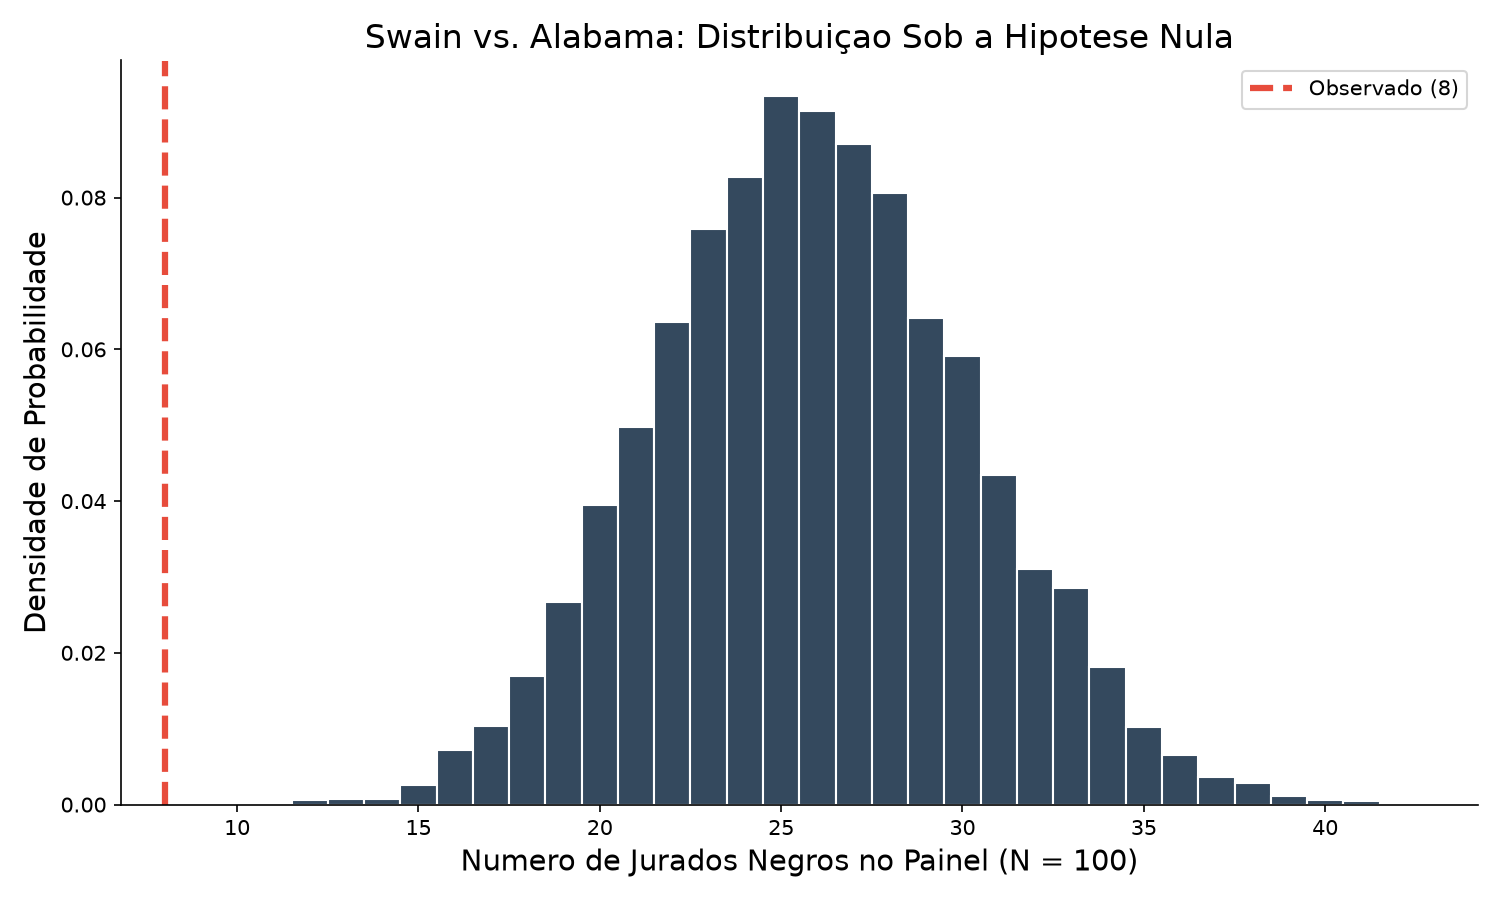
\includegraphics[width=\textwidth]{01_swain_histograma.png}
        \end{column}
    \end{columns}
\end{frame}

\section{Formalização e o Modelo de Mendel}

\begin{frame}{Definindo as Hipóteses}
    \begin{block}{Hipótese Nula ($H_0$)}
        Afirma que a variação observada nos dados é apenas fruto do acaso e não de uma causa sistemática. Sob essa hipótese, conseguimos simular computacionalmente a geração dos dados.
    \end{block}
    \begin{block}{Hipótese Alternativa ($H_1$)}
        Afirma que há um fator sistemático que gerou o desvio dos dados. A variação não pode ser explicada apenas pelo acaso.
    \end{block}
    \begin{alertblock}{Estatística de Teste}
        É a métrica quantitativa usada para avaliar quão longe os dados observados estão daquilo que é previsto pela hipótese nula $H_0$.
    \end{alertblock}
\end{frame}

\begin{frame}{Entendendo o P-Valor (Valor de Probabilidade)}
    \begin{block}{Definição Oficial}
        P-valor é a probabilidade de observar um valor de estatística de teste tão extremo ou mais extremo do que o observado, sob a premissa de que a Hipótese Nula $H_0$ é verdadeira.
    \end{block}
    \begin{alertblock}{Erros Comuns de Interpretação}
        \begin{itemize}
            \item \textbf{NÃO É} a probabilidade de a hipótese nula ser verdadeira.
            \item \textbf{NÃO É} a probabilidade de a hipótese alternativa ser falsa.
            \item É apenas um medidor de surpresa sob a hipótese nula.
        \end{itemize}
    \end{alertblock}
\end{frame}

\begin{frame}{Estudo de Caso: O Modelo de Genética de Mendel}
    \begin{block}{Mendel e a Hereditariedade das Plantas}
        Gregor Mendel propôs que em cruzamentos híbridos, a planta tinha $75\%$ de chance de ter flores roxas e $25\%$ de ter flores brancas.
    \end{block}
    \begin{columns}
        \begin{column}{0.5\textwidth}
            \textbf{Os Dados Observados:}
            \begin{itemize}
                \item Tamanho da amostra ($N$): $929$ plantas.
                \item Plantas de flor roxa: $705$ ($\approx 75.89\%$).
                \item Desvio observado: $0.89\%$.
            \end{itemize}
        \end{column}
        \begin{column}{0.5\textwidth}
            \centering
            \textit{Será que o desvio de $0.89\%$ da previsão de $75\%$ é sinal de falha do modelo de Mendel ou apenas ruído amostral?}
        \end{column}
    \end{columns}
\end{frame}

\begin{frame}{Matemática do Exemplo de Mendel}
    \begin{block}{Estatística de Teste: Distância Absoluta}
        Como há apenas duas categorias, a estatística de teste ideal é a diferença absoluta entre o percentual observado e $75\%$:
        $$\text{Estatística} = \left| \text{Percentual de Flores Roxas} - 75 \right|$$
    \end{block}
    \begin{block}{Cálculo do Valor Observado}
        $$\text{Percentual Observado} = \frac{705}{929} \times 100 \approx 75.888\%$$
        $$\text{Estatística Observada} = \left| 75.888 - 75 \right| = 0.888\%$$
    \end{block}
\end{frame}

\begin{frame}[fragile]{Abordagem Computacional: Mendel}
\begin{lstlisting}[language=Python]
import numpy as np

tamanho_amostra = 929
prob_roxa = 0.75
repeticoes = 10000

# Simula 10000 experimentos sob a hipotese nula
np.random.seed(42)
simulados = np.random.binomial(n=tamanho_amostra, p=prob_roxa, size=repeticoes)
percents_simulados = (simulados / tamanho_amostra) * 100
estatisticas_sim = np.abs(percents_simulados - 75.0)

# Calcula o P-valor
obs_dist = np.abs((705 / tamanho_amostra) * 100 - 75.0)
p_valor = np.count_nonzero(estatisticas_sim >= obs_dist) / repeticoes
print(f"P-valor: {p_valor:.4f}")
# Saida aproximada: 0.5418
\end{lstlisting}
\end{frame}

\begin{frame}{Mendel: Decisão Visual}
    \begin{columns}
        \begin{column}{0.5\textwidth}
            \textbf{Análise do Resultado:}
            \begin{itemize}
                \item O desvio de $0.888\%$ ou maior ocorre em mais de $54\%$ das simulações aleatórias.
                \item O desvio observado é comum no mundo nulo.
                \item \textbf{Decisão:} Não rejeitamos a hipótese nula $H_0$. O modelo de Mendel é consistente com os dados.
            \end{itemize}
        \end{column}
        \begin{column}{0.5\textwidth}
            \centering
            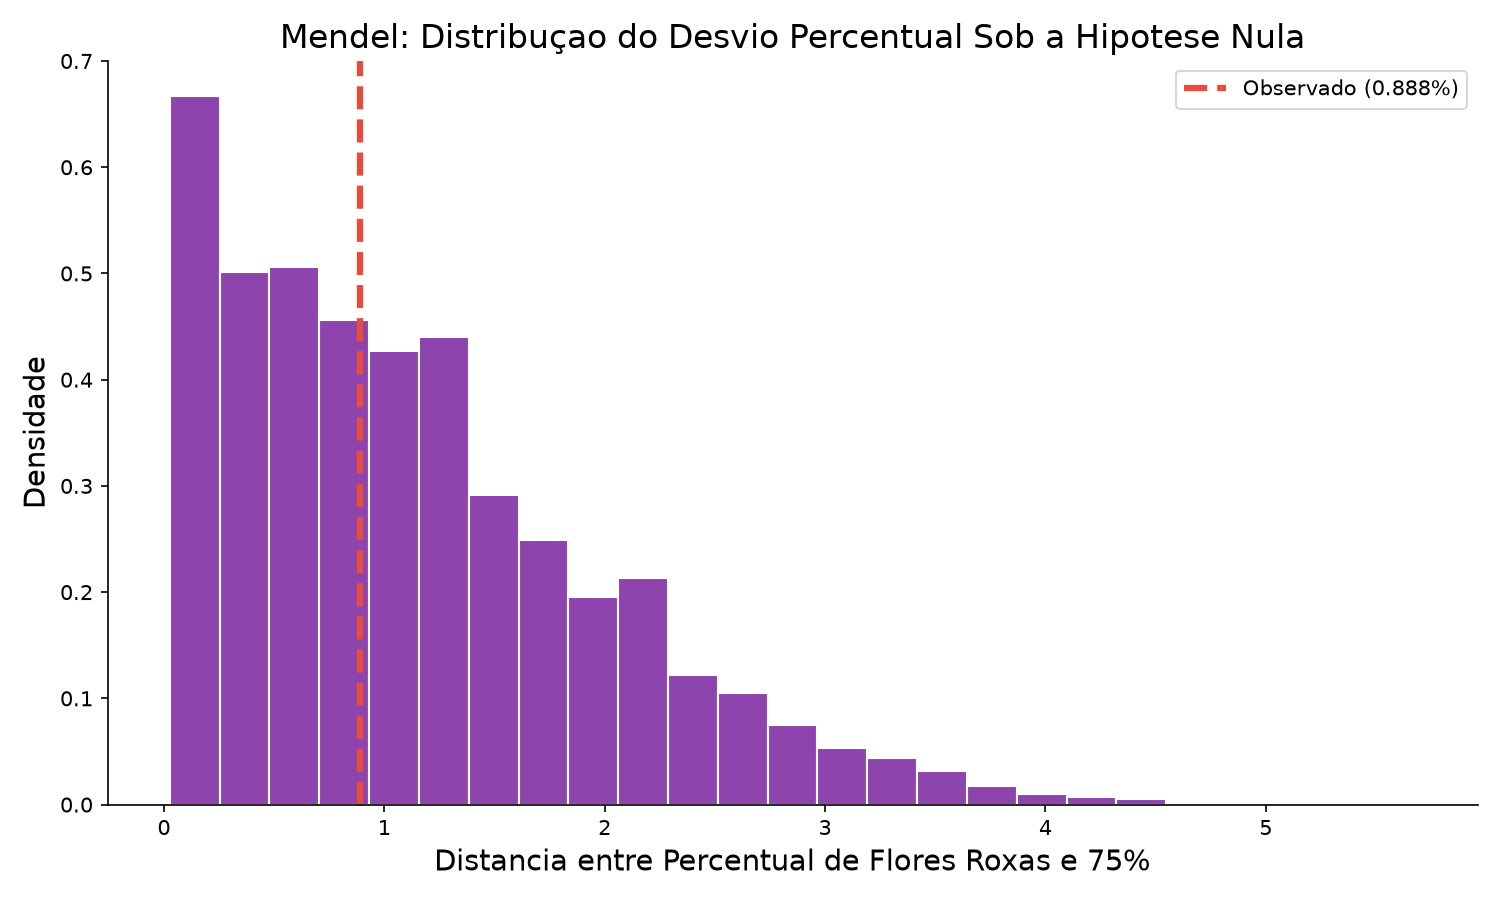
\includegraphics[width=\textwidth]{03_mendel_histograma.png}
        \end{column}
    \end{columns}
\end{frame}

\section{Múltiplas Categorias e TVD (Alameda County)}

\begin{frame}{Desafio de Múltiplas Categorias: Os Dados}
    \begin{block}{O Caso Alameda County (ACLU, 2010)}
        A ACLU avaliou o júri de 11 processos criminais ($1453$ pessoas no painel). É preciso determinar se a composição racial difere da população de forma sistemática.
    \end{block}
    
    \begin{columns}
        \begin{column}{0.48\textwidth}
            \begin{table}
                \centering
                \footnotesize
                \begin{tabular}{lcc}
                    \toprule
                    \textbf{Etnia} & \textbf{Elegível} & \textbf{Painel} \\
                    \midrule
                    Asiático & $0.15$ & $0.26$ \\
                    Negro & $0.18$ & $0.08$ \\
                    Branco & $0.54$ & $0.54$ \\
                    Hispânico & $0.12$ & $0.08$ \\
                    Outro & $0.01$ & $0.04$ \\
                    \bottomrule
                \end{tabular}
                \caption{Distribuição étnica}
            \end{table}
        \end{column}
        \begin{column}{0.52\textwidth}
            \centering
            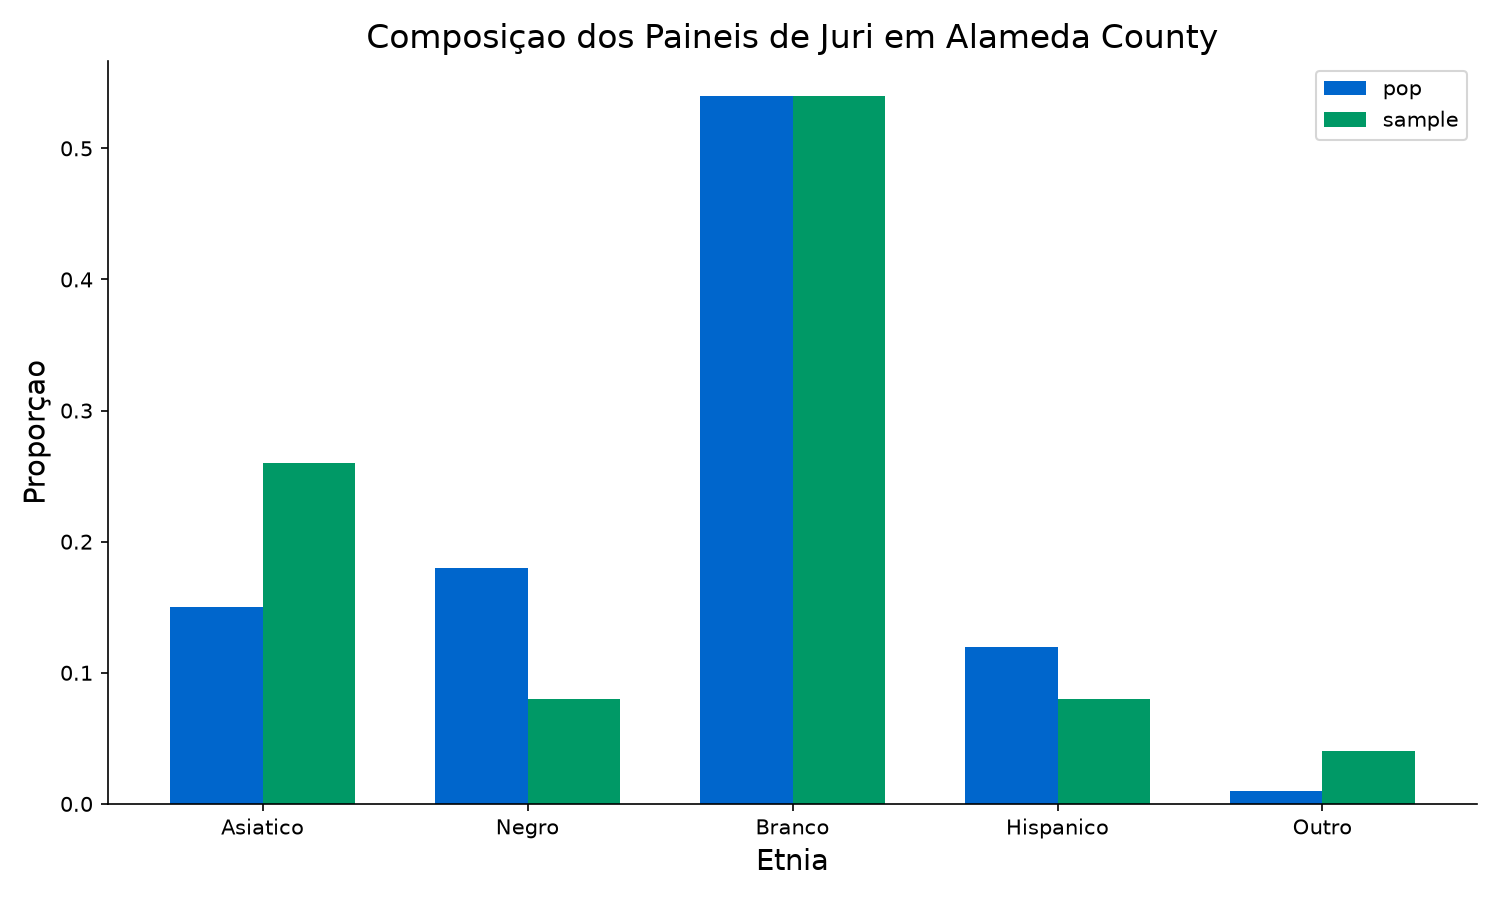
\includegraphics[width=\textwidth]{06_alameda_comparacao.png}
        \end{column}
    \end{columns}
\end{frame}

\begin{frame}{E se a Amostra Fosse Realmente Aleatória?}
    \begin{block}{Simulação de Seleção Justa (Amostra Multinomial)}
        Se o sorteio do júri de $1453$ pessoas fosse verdadeiramente aleatório e representativo, as proporções da amostra seriam muito próximas das proporções da população.
    \end{block}
    
    \begin{columns}
        \begin{column}{0.48\textwidth}
            \begin{table}
                \centering
                \footnotesize
                \begin{tabular}{lcc}
                    \toprule
                    \textbf{Etnia} & \textbf{Elegível} & \textbf{Aleatória} \\
                    \midrule
                    Asiático & $0.15$ & $0.14$ \\
                    Negro & $0.18$ & $0.18$ \\
                    Branco & $0.54$ & $0.56$ \\
                    Hispânico & $0.12$ & $0.11$ \\
                    Outro & $0.01$ & $0.01$ \\
                    \bottomrule
                \end{tabular}
                \caption{Amostra aleatória simulada}
            \end{table}
            \centering
            \vspace{0.1cm}
            {\footnotesize $TVD$ simulado: $0.0178$ ($1.78\%$)}
        \end{column}
        \begin{column}{0.52\textwidth}
            \centering
            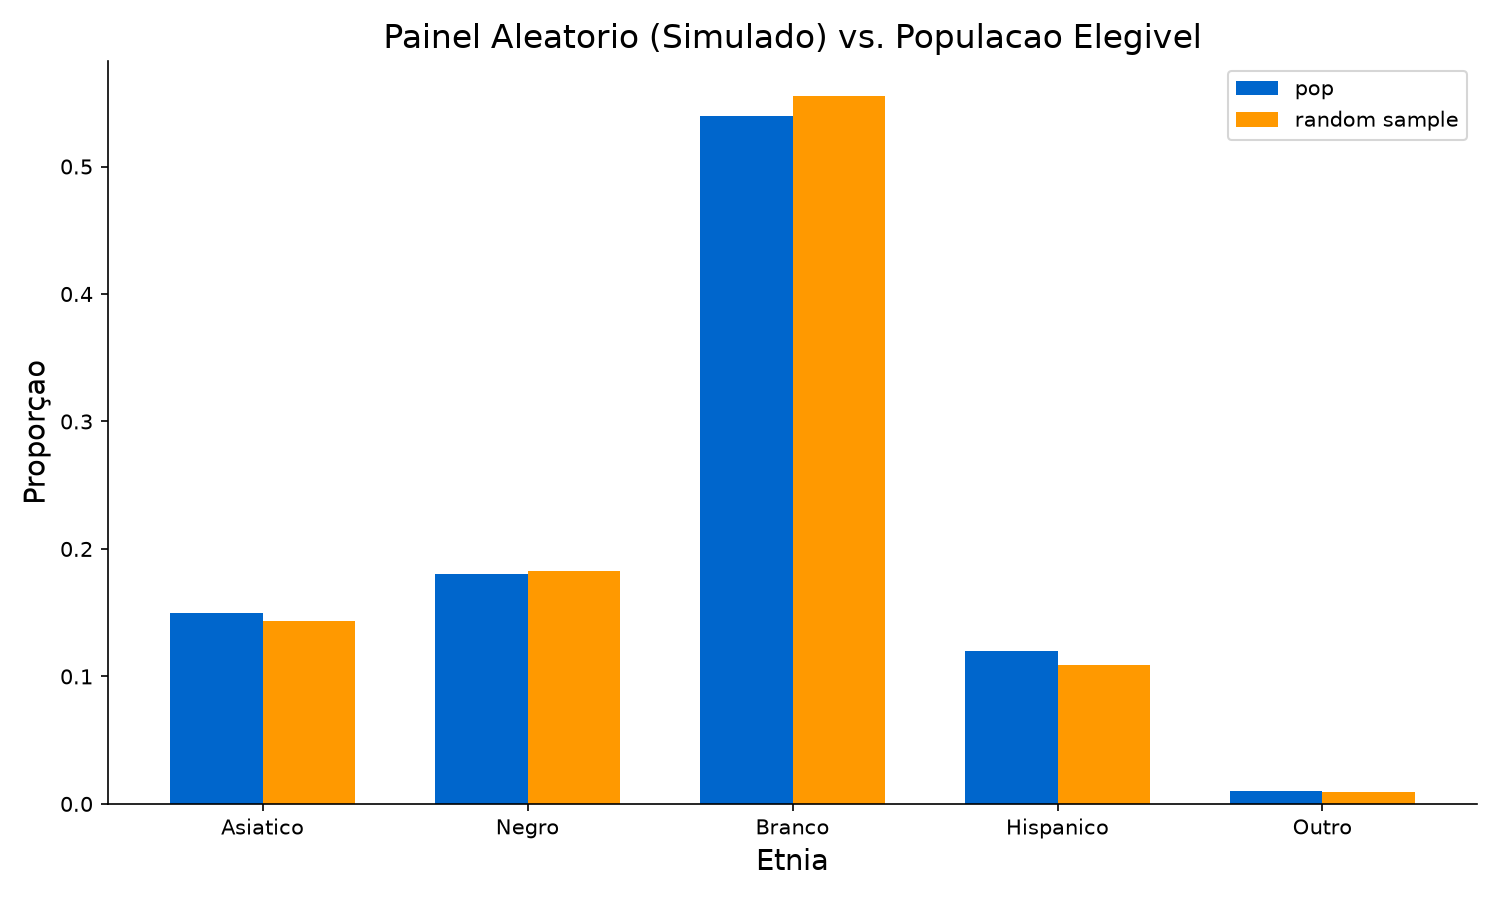
\includegraphics[width=\textwidth]{07_alameda_random_comparacao.png}
        \end{column}
    \end{columns}
\end{frame}

\begin{frame}{Matemática da Distância de Variação Total ($TVD$)}
    \begin{block}{Métrica de Distância de Variação Total ($TVD$)}
        Usada para comparar duas distribuições categóricas. É definida como metade da soma das diferenças absolutas entre as proporções de cada categoria:
        $$TVD = \frac{1}{2} \sum_{i=1}^{k} |p_i - q_i|$$
        Onde $p_i$ é a proporção amostral e $q_i$ é a proporção esperada.
    \end{block}
    \begin{block}{Exemplo de Cálculo para Alameda County:}
        {\small
        \begin{align*}
        TVD_{\text{obs}} = \frac{1}{2} \Big( &|0.26-0.15| + |0.08-0.18| + |0.54-0.54| + {} \\
        &|0.08-0.12| + |0.04-0.01| \Big) \\[1ex]
        TVD_{\text{obs}} = \frac{1}{2} \big( &0.11 + 0.10 + 0.00 + 0.04 + 0.03 \big) = \frac{0.28}{2} = 0.14
        \end{align*}
        }
    \end{block}
\end{frame}

\begin{frame}[fragile]{Abordagem Computacional: TVD}
\begin{lstlisting}[language=Python]
import numpy as np

prop_elegivel = np.array([0.15, 0.18, 0.54, 0.12, 0.01])
prop_painel = np.array([0.26, 0.08, 0.54, 0.08, 0.04])
obs_tvd = 0.5 * np.sum(np.abs(prop_painel - prop_elegivel))

tvds = []
np.random.seed(42)
for _ in range(10000):
    # Sorteia 1453 jurados de acordo com a distribuicao populacional
    amostra = np.random.multinomial(1453, prop_elegivel)
    prop_sim = amostra / 1453
    tvd_sim = 0.5 * np.sum(np.abs(prop_sim - prop_elegivel))
    tvds.append(tvd_sim)

# Calcula o P-valor
p_valor = np.count_nonzero(tvds >= obs_tvd) / 10000
print(f"P-valor: {p_valor}")
# Saida esperada: 0.0
\end{lstlisting}
\end{frame}

\begin{frame}{Alameda County: Decisão Visual}
    \begin{columns}
        \begin{column}{0.5\textwidth}
            \textbf{Análise do Gráfico:}
            \begin{itemize}
                \item Sob a hipótese nula, o $TVD$ máximo gerado em $10.000$ repetições foi próximo de $0.05$.
                \item O valor observado de $0.14$ está fora da região de variação aceitável do acaso.
                \item \textbf{Decisão:} Rejeitamos a hipótese nula $H_0$. O painel de Alameda County não foi selecionado aleatoriamente.
            \end{itemize}
        \end{column}
        \begin{column}{0.5\textwidth}
            \centering
            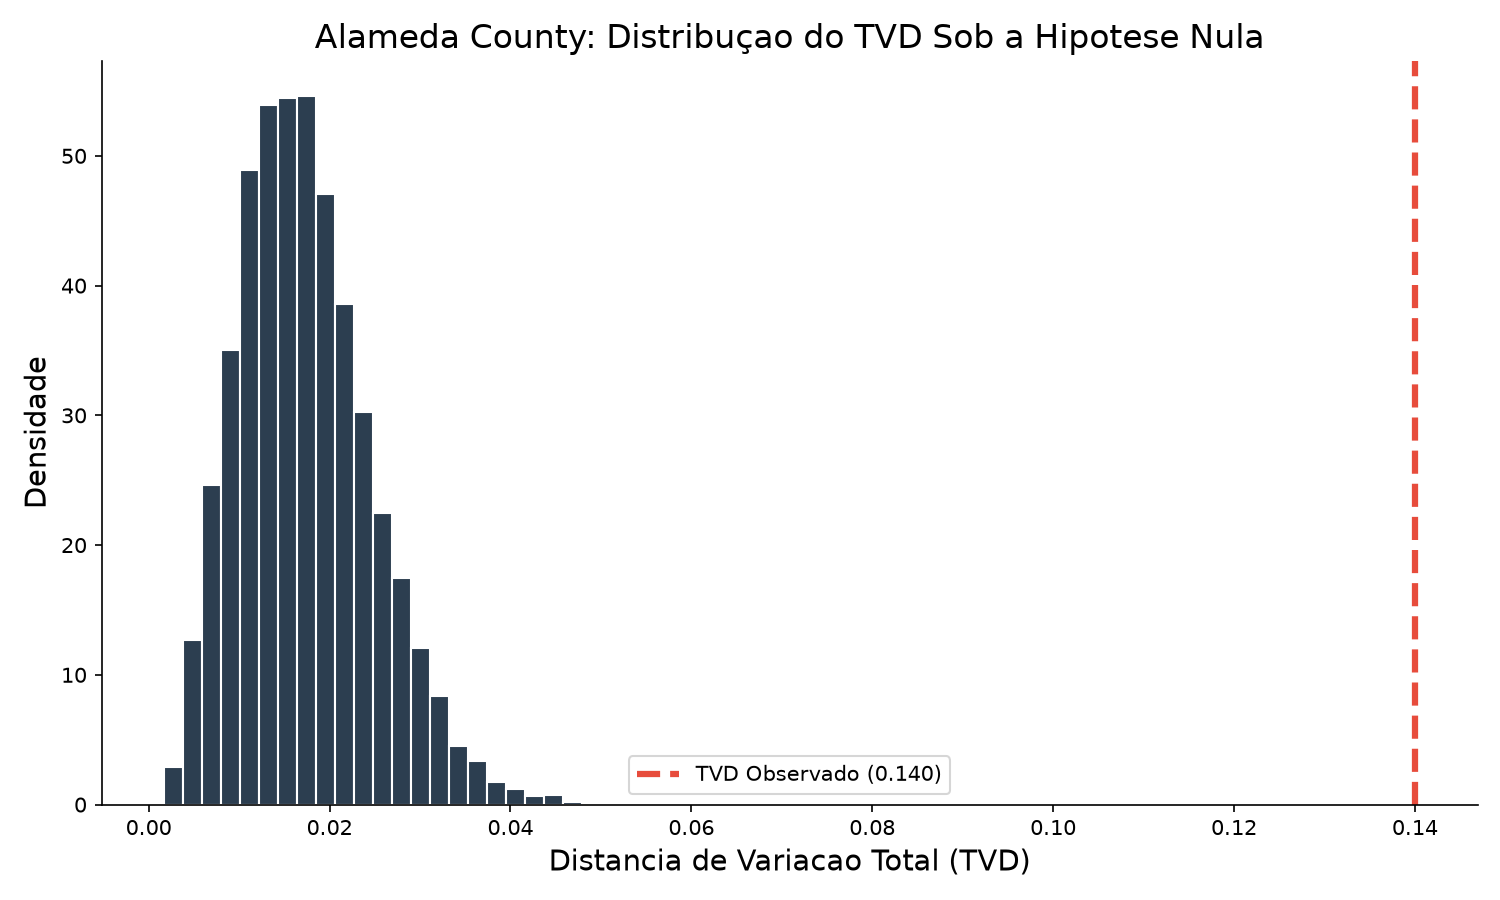
\includegraphics[width=\textwidth]{02_alameda_tvd.png}
        \end{column}
    \end{columns}
\end{frame}

\section{Testes A/B e Permutação}

\begin{frame}{Testes A/B e a Lógica de Permutação}
    \begin{block}{A Lógica da Permutação de Rótulos}
        Se a hipótese nula $H_0$ é verdadeira (não há diferença entre o grupo de Tratamento e Controle), a associação entre as variáveis é irrelevante. Logo, podemos embaralhar aleatoriamente os rótulos dos grupos sem alterar a estrutura básica dos dados.
    \end{block}
    \begin{block}{Algoritmo Geral:}
        \begin{enumerate}
            \item Reúna os dados dos dois grupos em um único vetor.
            \item Embaralhe aleatoriamente os elementos.
            \item Separe a primeira amostra com tamanho $N_A$ (grupo A) e a segunda com $N_B$ (grupo B).
            \item Calcule a diferença de médias.
            \item Repita o processo $10.000$ vezes para criar a distribuição nula.
        \end{enumerate}
    \end{block}
\end{frame}

\begin{frame}{Caso 1: Tabagismo Materno e Peso do Bebê}
    \begin{block}{Pergunta Científica}
        O tabagismo de gestantes afeta o peso do recém-nascido?
    \end{block}
    \begin{columns}
        \begin{column}{0.5\textwidth}
            \textbf{Detalhes dos Grupos:}
            \begin{itemize}
                \item Grupo A (Fumantes): $459$ bebês.
                \item Grupo B (Não Fumantes): $715$ bebês.
                \item Estatística: $\bar{X}_B - \bar{X}_A$
                \item Diferença de médias observada: $0.26$ kg.
            \end{itemize}
        \end{column}
        \begin{column}{0.5\textwidth}
            \centering
            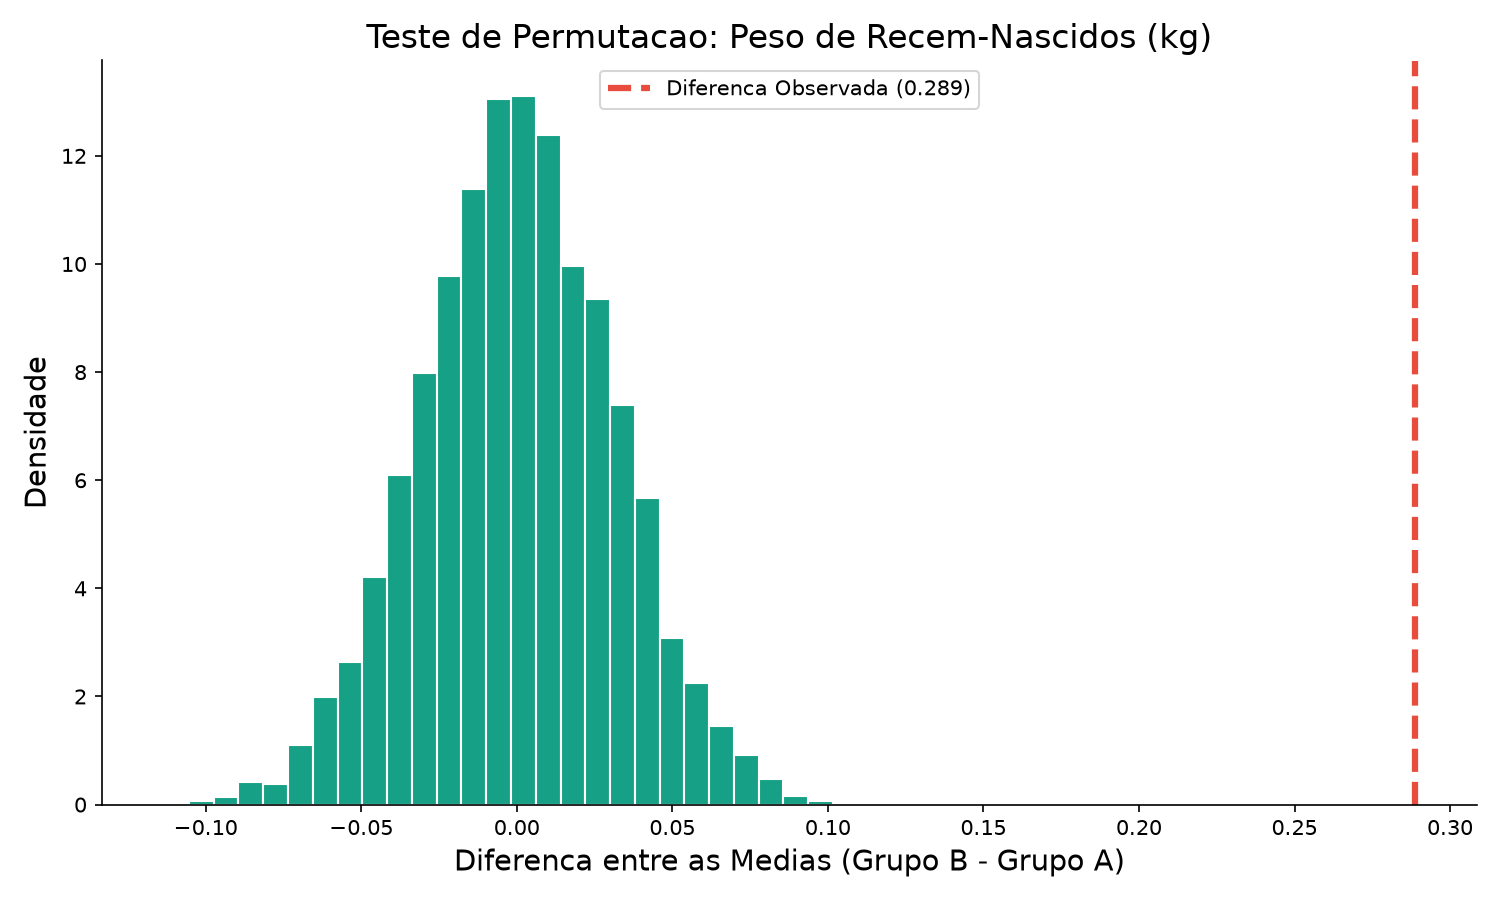
\includegraphics[width=\textwidth]{04_permutacao_peso.png}
        \end{column}
    \end{columns}
\end{frame}

\begin{frame}[fragile]{Código em Python: Permutação de Peso de Bebês}
\begin{lstlisting}[language=Python]
import numpy as np

conjunto = np.concatenate([grupo_fumantes, grupo_nao_fumantes])
n_a = len(grupo_fumantes)
diferencas = []
np.random.seed(42)

for _ in range(10000):
    # Embaralha os pesos de todos os bebes
    embaralhado = np.random.permutation(conjunto)
    sim_a = embaralhado[:n_a]
    sim_b = embaralhado[n_a:]
    diferencas.append(np.mean(sim_b) - np.mean(sim_a))

# Calcula o P-valor
p_valor = np.count_nonzero(diferencas >= 0.26) / 10000
print(f"P-valor: {p_valor:.4f}")
# Saida: 0.0000
\end{lstlisting}
\end{frame}

\begin{frame}{Simulação no Modelo Nulo e Caudas do Teste}
    \begin{block}{O que significa ``ser mais extremo''?}
        Dependendo de como definimos a nossa \textbf{Hipótese Alternativa ($H_1$)}, medimos o desvio em caudas diferentes da distribuição:
        \begin{enumerate}
            \item \textbf{Unilateral (Cauda Direita):} $\text{Média}_{\text{Não-Fumante}} > \text{Média}_{\text{Fumante}}$
            \begin{itemize}
                \item Buscamos proporção de valores simulados $\geq 0.26$ kg.
            \end{itemize}
            \item \textbf{Unilateral (Cauda Esquerda):} $\text{Média}_{\text{Não-Fumante}} < \text{Média}_{\text{Fumante}}$
            \begin{itemize}
                \item Buscamos proporção de valores simulados $\leq 0.26$ kg.
            \end{itemize}
            \item \textbf{Bicaudal (Duas Caudas):} $\text{Média}_{\text{Não-Fumante}} \neq \text{Média}_{\text{Fumante}}$
            \begin{itemize}
                \item Buscamos proporção de valores em módulo $|\text{simulado}| \geq 0.26$ kg.
            \end{itemize}
        \end{enumerate}
    \end{block}
    \centering
    \textit{Cada alternativa altera a área (cauda) que calculamos para obter o P-valor.}
\end{frame}

\begin{frame}{Decisão Estatística: Peso de Bebês}
    \begin{block}{Resultado Obtido}
        \begin{itemize}
            \item Diferença de médias observada na amostra real: $0.26$ kg.
            \item Em $10.000$ embaralhamentos (permutações) simulados sob a hipótese nula $H_0$, a diferença de médias nunca alcançou $0.26$ kg.
            \item Nosso $p$-valor empírico foi de $0.0000$ ($0\%$).
        \end{itemize}
    \end{block}
    \begin{alertblock}{Tomada de Decisão}
        Como $p$-valor ($0\%$) $<$ Limiar de Significância ($\alpha = 5\%$), \textbf{rejeitamos a hipótese nula $H_0$}.
    \end{alertblock}
    \centering
    \textbf{Conclusão:} O tabagismo na gestação está estatisticamente associado a uma redução sistemática no peso do recém-nascido. A diferença não é explicável pelo acaso.
\end{frame}

\begin{frame}{Caso 2: Salários NBA (Cleveland vs. Houston)}
    \begin{block}{O Problema de Variância}
        Cleveland Cavs e Houston Rockets têm salários médios aparentando diferença ($10.23$ M\$ vs $7.10$ M\$ na população). Porém, a variância de salários na NBA é extremamente alta e a amostra de jogadores disponível é muito pequena ($N = 15$ por time).
    \end{block}
    \begin{block}{Amostra Simulada ($N=15$)}
        Para ilustrar o teste computacionalmente, geramos uma amostra sintética de $15$ jogadores por time:
        \begin{itemize}
            \item Média Cleveland na Amostra: $10.34$ M\$
            \item Média Houston na Amostra: $2.85$ M\$
            \item Diferença Observada na Amostra: $7.50$ M\$
        \end{itemize}
    \end{block}
    \centering
    \textit{Será que uma diferença aparente de $7.50$ M\$ é significativa ou pode ser explicada apenas pela variabilidade natural dos salários?}
\end{frame}

\begin{frame}{Resultados de Permutações nos Salários}
    \begin{block}{Médias de Cleveland e Houston após o Shuffle}
        Sob a hipótese nula $H_0$, a designação do time é mero rótulo. Ao misturar todos os salários e sorteá-los em dois grupos de 15, veja como as médias variam por puro acaso:
    \end{block}
    
    \begin{table}
        \centering
        \small
        \begin{tabular}{lccc}
            \toprule
            \textbf{Rodada (Shuffle)} & \textbf{Média Cleveland} & \textbf{Média Houston} & \textbf{Diferença ($C - H$)} \\
            \midrule
            Amostra Real Simulada & $10.34$ M\$ & $2.85$ M\$ & $7.50$ M\$ \\
            \midrule
            Simulação 1 & $7.92$ M\$ & $5.27$ M\$ & $2.64$ M\$ \\
            Simulação 2 & $4.79$ M\$ & $8.40$ M\$ & $-3.61$ M\$ \\
            Simulação 3 & $9.13$ M\$ & $4.06$ M\$ & $5.08$ M\$ \\
            Simulação 4 & $5.23$ M\$ & $7.96$ M\$ & $-2.74$ M\$ \\
            \bottomrule
        \end{tabular}
        \caption{Exemplos de médias e diferenças após permutações}
    \end{table}
    \centering
    \textit{Note que mesmo no modelo nulo (sem efeito real), as diferenças flutuam bastante devido à alta variabilidade dos dados.}
\end{frame}

\begin{frame}[fragile]{Código em Python: Salários da NBA}
\begin{lstlisting}[language=Python]
import numpy as np

conjunto = np.concatenate([grupo_houston, grupo_cleveland])
n_a = len(grupo_houston)
diferencas_nba = []
np.random.seed(42)

for _ in range(10000):
    # Embaralha os salarios dos jogadores
    embaralhado = np.random.permutation(conjunto)
    sim_a = embaralhado[:n_a]
    sim_b = embaralhado[n_a:]
    diferencas_nba.append(np.mean(sim_b) - np.mean(sim_a))

# Teste bicaudal para o P-valor
obs_diff = 7.50
p_valor = np.count_nonzero(np.abs(diferencas_nba) >= np.abs(obs_diff)) / 10000
print(f"P-valor bicaudal: {p_valor:.4f}")
# Saida: 0.1010
\end{lstlisting}
\end{frame}

\begin{frame}{Decisão Estatística: Salários da NBA}
    \begin{columns}
        \begin{column}{0.5\textwidth}
            \textbf{Análise do P-valor Bicaudal:}
            \begin{itemize}
                \item Diferença de médias na amostra: $7.50$ M\$.
                \item P-valor bicaudal: $10.10\%$.
                \item Como $p\text{-valor} \geq 5\%$, \textbf{não rejeitamos a hipótese nula $H_0$}.
            \end{itemize}
            \vspace{0.2cm}
            \textbf{Conclusão:} A diferença observada nos salários não é estatisticamente significante; a alta variação salarial combinada com a amostra pequena torna a diferença explicável pelo acaso.
        \end{column}
        \begin{column}{0.5\textwidth}
            \centering
            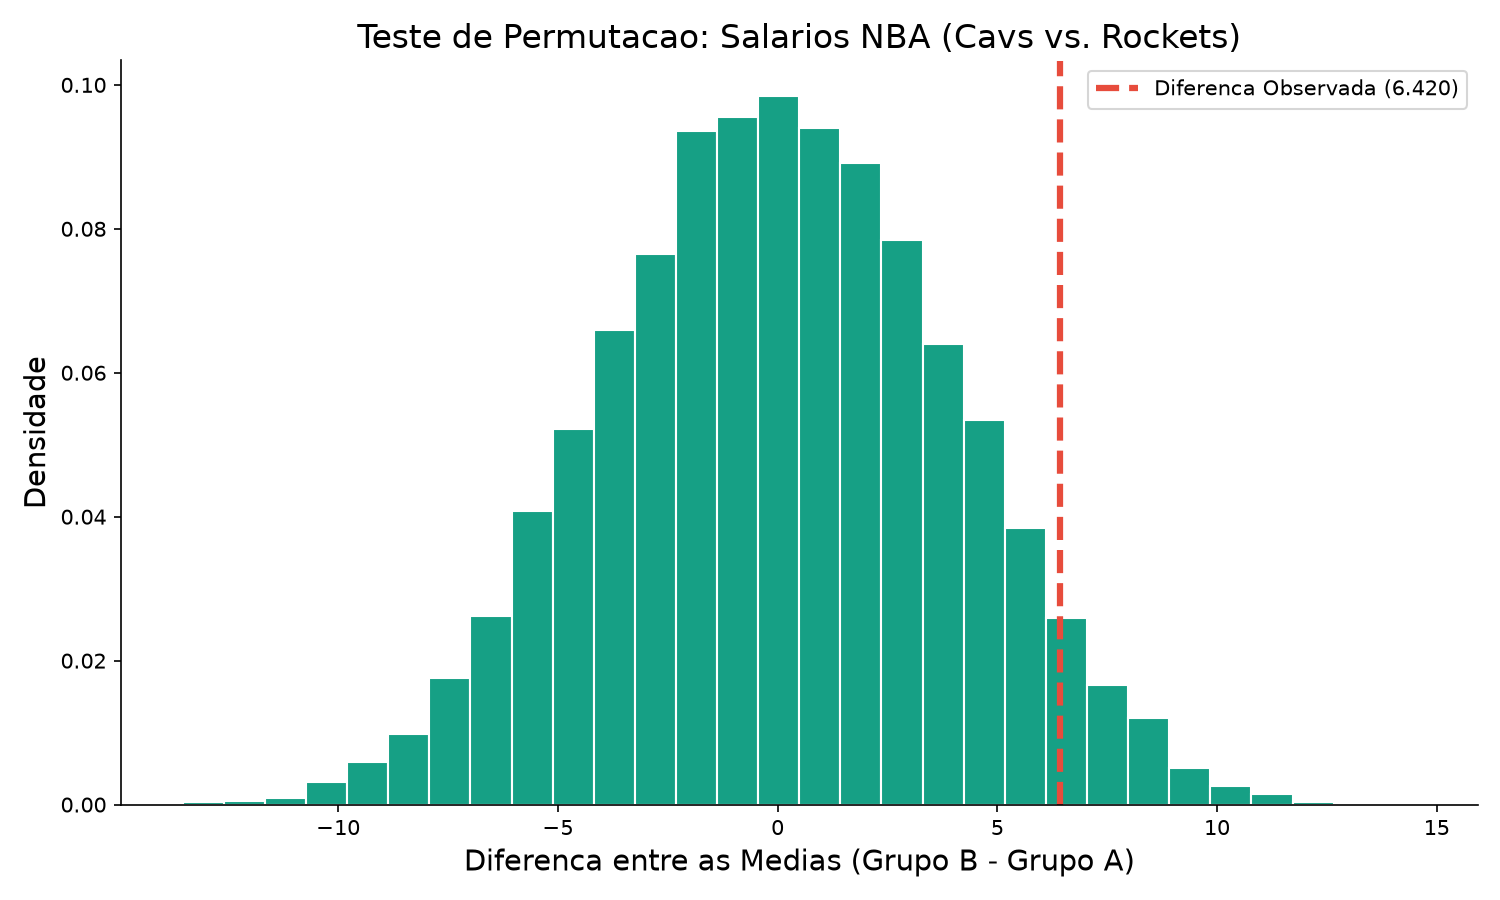
\includegraphics[width=\textwidth]{05_permutacao_nba.png}
        \end{column}
    \end{columns}
\end{frame}

\section{Limites de Significância e Erros de Decisão}

\begin{frame}{O Limiar de Significância e Sir Ronald Fisher}
    \begin{block}{A Convenção de 5\%}
        Sir Ronald Fisher publicou em 1925 que o limiar de 5\% ($\alpha = 0.05$) é conveniente para julgar se um desvio deve ou não ser considerado significativo.
    \end{block}
    \begin{alertblock}{Cuidado com o Limiar}
        \begin{itemize}
            \item Trata-se de uma convenção histórica, não uma verdade matemática absoluta.
            \item Em conjuntos de dados muito grandes, é recomendável buscar limites muito menores (ex: $0.01$ ou $0.001$) para evitar falsos positivos.
            \item Cuidado com a prática do ``P-hacking'' (manipulação de dados até atingir o $p < 0.05$).
        \end{itemize}
    \end{alertblock}
\end{frame}

\begin{frame}{Erros de Decisão Estatística}
    \begin{block}{Erro do Tipo I (Falso Positivo)}
        Ocorre quando rejeitamos a Hipótese Nula $H_0$, embora ela seja verdadeira. A probabilidade máxima de cometer esse erro é igual ao nível de significância $\alpha$.
    \end{block}
    \begin{block}{Erro do Tipo II (Falso Negativo)}
        Ocorre quando falhamos em rejeitar a Hipótese Nula $H_0$, embora a Hipótese Alternativa $H_1$ seja verdadeira. A probabilidade desse erro é representada por $\beta$.
    \end{block}
    \begin{alertblock}{Poder do Teste}
        Representado por $1 - \beta$, é a capacidade do teste estatístico de detectar um sinal real quando ele realmente existe.
    \end{alertblock}
\end{frame}

\begin{frame}{Matriz de Decisão Estatística}
    \begin{table}
        \centering
        \footnotesize
        \begin{tabular}{lcc}
            \toprule
            \textbf{Realidade} & \textbf{Decisão: Não Rejeitar $H_0$} & \textbf{Decisão: Rejeitar $H_0$} \\
            \midrule
            $H_0$ é Verdadeira & Decisão Correta & \textbf{Erro Tipo I} ($\alpha$ Falso Positivo) \\ \addlinespace
            $H_1$ é Verdadeira & \textbf{Erro Tipo II} ($\beta$ Falso Negativo) & Decisão Correta (Poder: $1-\beta$) \\
            \bottomrule
        \end{tabular}
        \caption{Matriz de decisão e probabilidades de erro}
    \end{table}
    \centering
    \textit{Existe um compromisso entre $\alpha$ e $\beta$: diminuir a tolerância a falsos positivos ($\alpha$) tipicamente reduz o poder do teste, aumentando os falsos negativos ($\beta$).}
\end{frame}

\begin{frame}{Resumo e Principais Aprendizados}
    \begin{block}{Pontos-Chave da Aula}
        \begin{itemize}
            \item \textbf{Modelo Nulo:} O modelo do acaso no qual conseguimos realizar simulações computacionais.
            \item \textbf{TVD:} Estatística de teste robusta para comparar distribuições com múltiplas categorias.
            \item \textbf{Teste de Permutação:} Método de reamostragem ideal para Testes A/B, pois não exige premissas distributivas.
            \item \textbf{P-Valor:} Mede a compatibilidade entre a amostra observada e o modelo nulo.
        \end{itemize}
    \end{block}
    \centering
    \textbf{Dica:} Sempre comece definindo com clareza a Hipótese Nula ($H_0$) e a Estatística de Teste apropriada!
\end{frame}

\begin{frame}{Referências Bibliográficas}
    \begin{block}{Leituras Recomendadas}
        \footnotesize
        \begin{itemize}
            \item \textbf{Learning Data Science} \\
            Sam Lau, Joey Gonzalez, and Deb Nolan. \\
            Capítulo 17: Inference, Prediction, and Generalization. \\
            \url{https://learningds.org/ch/17/inf_pred_gen_HT.html}
            \vspace{0.3cm}
            \item \textbf{Computational and Inferential Thinking} \\
            Ani Adhikari and John DeNero. \\
            Capítulo 11: Testing Hypotheses. \\
            \url{https://inferentialthinking.com/chapters/11/testing-hypotheses/}
        \end{itemize}
    \end{block}
\end{frame}



\end{document}
